\documentclass[../DoAn.tex]{subfiles}
\begin{document}

\section{Thiết kế kiến trúc}
\subsection{Lựa chọn kiến trúc phần mềm}

Hình \ref{fig:Fig1} mô tả kiến trúc tổng quan hệ thống điều khiển xe Arduino qua ứng dụng Flutter. Hệ thống dựa trên kiến trúc DDD (Domain-Driven Design) và thêm một lớp khác để phục vụ cho việc phát triển và bảo trì.

\begin{figure}[H]
    \centering
    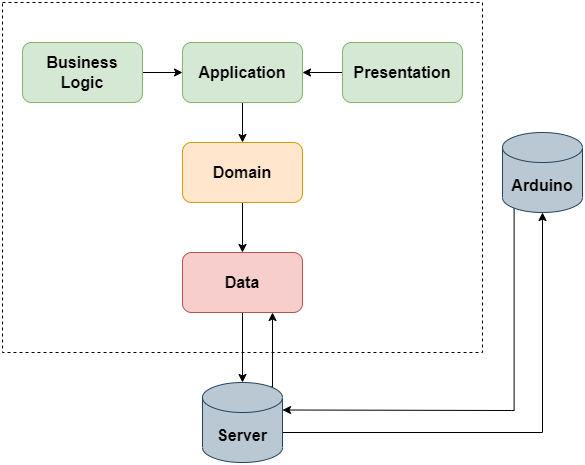
\includegraphics[scale = 0.6]{Hinhve/uml_package.png}
    \caption{Kiến trúc tổng quan hệ thống IoT}
    \label{fig:Fig1}
\end{figure}

Trong kiến trúc này, Business Logic sẽ đảm nhiệm vai trò quản lý các trạng thái của dữ liệu, lớp này giữ các trạng thái thay đổi của các Model được repository cung cấp. Lớp Presentation đóng vai trò kết xuất các trạng thái thành các thành phần và hiển thị dữ liệu lên màn hình cho người dùng. Tiếp theo, lớp Domain phụ trách chuyển đổi dữ liệu thành các lớp dữ liệu, các dữ liệu thô sẽ được chuyển đổi thành mô hình riêng và lớp Business Logic sẽ tiếp nhận mô hình đó. Cuối cùng, lớp data là lớp sẽ giao tiếp với các API, lấy dữ liệu về.

\subsection{Thiết kế tổng quan}

Ở phần 4.1, chương này trình bày về thiết kế phần mềm của hệ thống IoT, tương ứng với thiết kế phần mềm tổng quan đó, hình \ref{fig:Fig2} thể hiện biểu đồ gói của ứng dụng điều khiển thiết bị Arduino.

\begin{figure}[H]
    \centering
    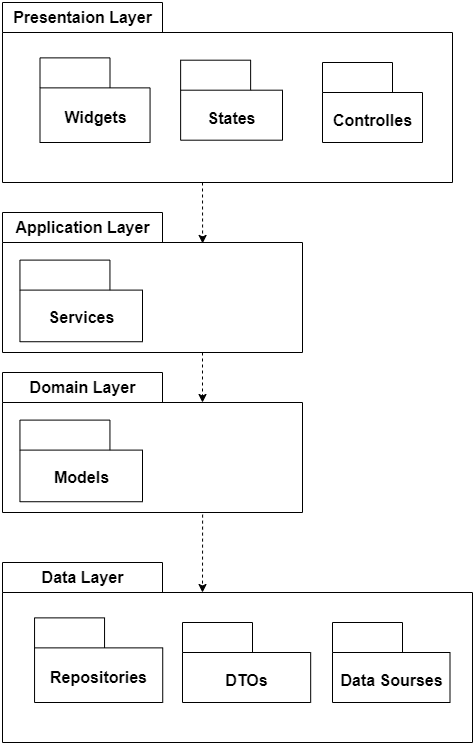
\includegraphics[scale = 0.6]{Hinhve/UML_tong_quan.png}
    \caption{Thiết kế tổng quan ứng dụng điều khiển IoT}
    \label{fig:Fig2}
\end{figure}

Thiết kế tổng quan bao gồm 4 tầng: (i) tầng trình diễn trên cùng bao gồm các gói Widgets chứa giao diện ứng dụng, gói States chứa các trạng thái của các widgets trong ứng dụng Flutter và gói Controllers là nơi tiếp nhận các yêu cầu từ gói States, xử lý và gửi tới gói tiếp theo, (ii) tầng ứng dụng chỉ chứa gói Services để tiếp nhận, xử lý các yêu cầu của người dùng từ tầng trình diễn và lấy dữ liệu của tầng miền, (iii) tầng miền chứa gói models có nhiệm vụ chuyển đổi dữ liệu thô thành mô hình để các gói phía trên xử lý được và nhận dữ liệu từ tầng ứng dụng, (iv) tầng dữ liệu là nơi tiếp nhận dữ liệu thô từ APIs hoặc cơ sở dữ liệu.

\subsection{Thiết kế chi tiết gói}

\subsubsection{Thiết kế chi tiết gói Presentation}

\begin{figure}[H]
    \centering
    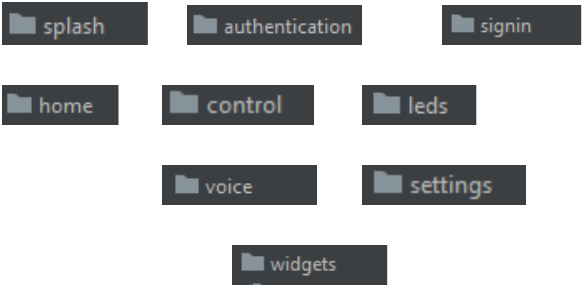
\includegraphics[scale = 0.6]{Hinhve/package_presentation.png}
    \caption{Thiết kế chi tiết gói Presentation}
    \label{fig:0.1.3.1}
\end{figure}

Hình \ref{fig:0.1.3.1} là thiết kế các gói con trong gói Presentation, mỗi gói con sẽ thực hiện chức năng riêng về mặt giao diện trong hệ thống. 

Gói Authentication chứa các màn hình liên quan đến đăng nhập, đăng ký và các màn trước khi đăng nhập. Gói Control có các màn hình liên quan tới việc điều khiển xe, gói Leds chứa các màn hình về điều khiển đèn LED, gói Voice bao quát cho các chức năng liên quan đến giọng nói và gói Settings sẽ liên quan tới những cài đặt trong ứng dụng, cài đặt để cho xe chạy với những giá trị khác nhau.

\subsubsection{Thiết kế chi tiết gói Data}

\begin{figure}[H]
    \centering
    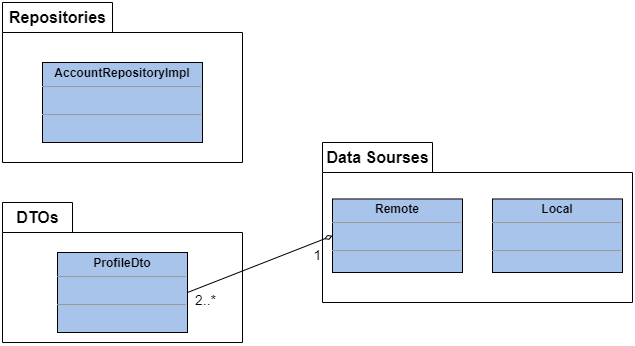
\includegraphics[scale = 0.6]{Hinhve/package_data.png}
    \caption{Thiết kế chi tiết gói Data}
    \label{fig:0.1.3.2}
\end{figure}

Hình \ref{fig:0.1.3.2} mô tả chi tiết các lớp trong gói Data. Trong gói Data Sources có 2 lớp, lớp Remote là nơi nhận dữ liệu về truyền dữ liệu lên bằng các phương thức khác nhau như API, Firebase\cite{Firebase}, ..., còn lớp Local chịu trách nhiệm xử lý những dữ liệu ở dưới ứng dụng, chạy trong vòng đời của ứng dụng. Gói DTOs chứa nhiều lớp như ProfileDto, ở đây các lớp này sẽ xử lý các trường dữ liệu về. Lớp Remote được hình thành từ nhiều lớp Dto hợp thành. Gói Repositories chứa các lớp như AccountReposityImpl dùng để thực thi dữ liệu, lớp này phụ thuộc vào các lớp Dto tương ứng.

\subsubsection{Thiết kế chi tiết gói Domain}

\begin{figure}[H]
    \centering
    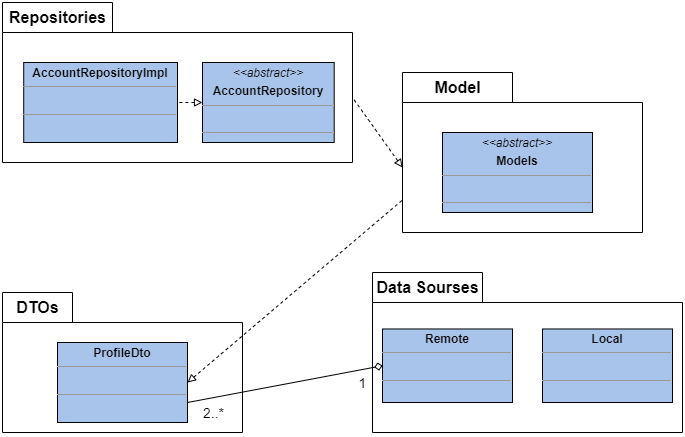
\includegraphics[scale = 0.6]{Hinhve/package_data_domain.png}
    \caption{Thiết kế chi tiết gói Domain}
    \label{fig:0.1.3.3}
\end{figure}

Hình \ref{fig:0.1.3.3} mô tả chi tiết các lớp trong gói Domain và liên kết với gói Data. Hai lớp Models và AccountRepository là các lớp abstract giữ nhiệm vụ giao tiếp dữ liệu với phía Presentation, bên cạnh đó lớp Dtos sẽ phụ thuộc vào 
lớp Models, Models thông qua lớp Dto để lấy dữ liệu, xử lý và biến đổi phù hợp với gói Presentaion còn Repository sẽ là các hàm chức năng giúp gói Presentaion thực thi.

\section{Thiết kế chi tiết}
\subsection{Thiết kế giao diện}

\subsubsection{Thông tin màn hình}

Hệ thống ứng dụng điều khiển thiết bị Arduino được xây dựng trên đa nền tảng đó là Android, iOS và Web. Đối với Android, ứng dụng chạy tốt và phù hợp với các thiết bị nhiều kích thước kể cả Tablet, còn iOS ứng dụng cũng có thể chạy trên cả iPad mà không bị vỡ giao diện, vẫn đem lại trải nghiệm tốt. Về nền tảng website, ứng dụng hỗ trợ trình duyệt Chrome đa kích thước

\subsubsection{Thiết kế các màn hình}

Thiết kế các chi tiết trong màn hình được thống nhất qua các nút, tiêu đề, màu sắc, nơi nhập thông tin, ... .

\begin{figure}[H]
    \centering
    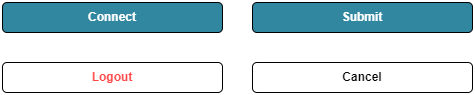
\includegraphics[scale = 0.75]{Hinhve/button.png}
    \caption{Thiết kế các nút nhấn}
    \label{fig:Fig4}
\end{figure}

\begin{figure}[H]
    \centering
    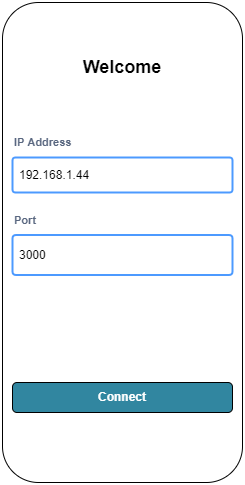
\includegraphics[scale = 0.75]{Hinhve/form.png}
    \caption{Thiết kế form điền thông tin và xác nhận}
    \label{fig:Fig5}
\end{figure}

\begin{figure}[H]
    \centering
    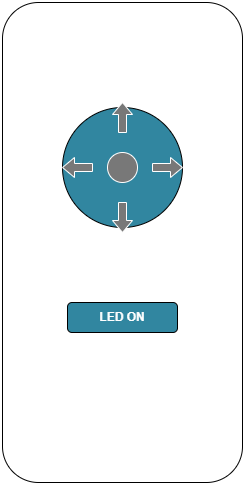
\includegraphics[scale = 0.75]{Hinhve/control.png}
    \caption{Thiết kế màn hình điều khiển xe Arduino}
    \label{fig:Fig6}
\end{figure}

\begin{figure}[H]
    \centering
    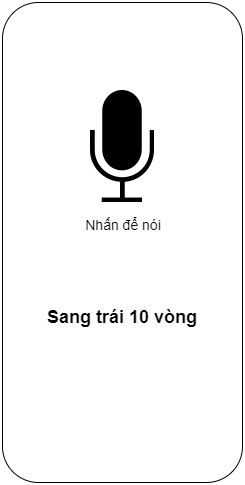
\includegraphics[scale = 0.75]{Hinhve/voice_control.png}
    \caption{Thiết kế màn hình điều khiển bằng giọng nói}
    \label{fig:Fig7}
\end{figure}

\subsection{Thiết kế lớp}
 Trong phần này, em sẽ trình bày một số thiết kế luồng cho các use case quan trọng.

 \begin{figure}[H]
    \centering
    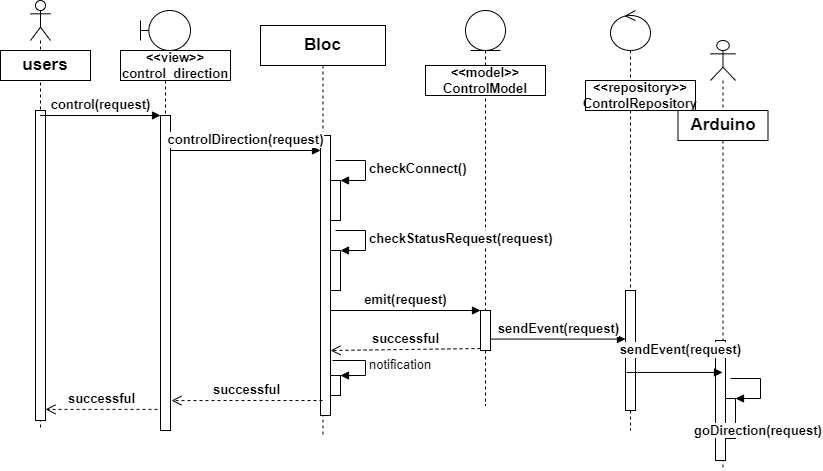
\includegraphics[scale = 0.5]{Hinhve/sequence_dieu_khien_xe.png}
    \caption{Biểu đồ trình tự điều khiển xe}
    \label{fig:4.2.2.1}
\end{figure}

Hình \ref{fig:4.2.2.1} thể hiện luồng điều khiển xe di chuyển các hướng. Sau khi kết nối được với server, người dùng di chuyển bộ điều khiển theo hướng muốn chọn. Tại tầng Bloc sẽ kiểm tra kết nối với server trước, tiếp đó sẽ gửi tín hiệu với ControlModel, qua ControlRepository để gửi sự kiện tới xe Arduino. Arduino lắng nghe sự kiện, nếu sự kiện đúng theo mã đã lập trình, xe thực hiện di chuyển theo hàm goDirection().

 \begin{figure}[H]
    \centering
    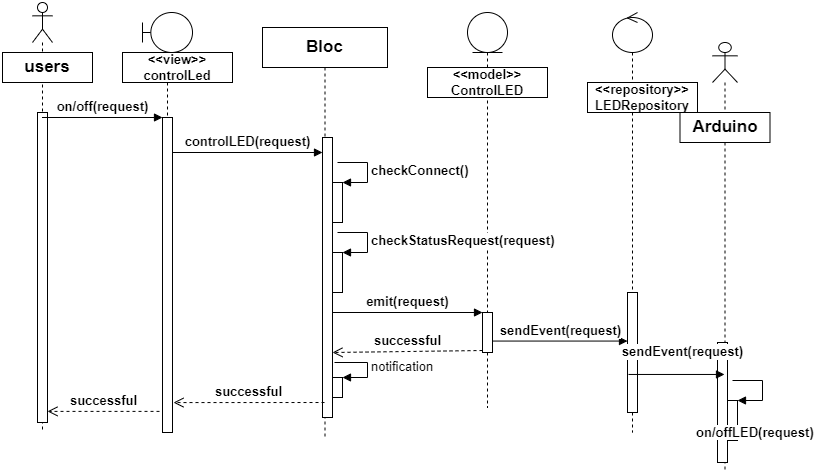
\includegraphics[scale = 0.5]{Hinhve/sequence_dieu_khien_led.png}
    \caption{Biểu đồ trình tự điều khiển đèn LED}
    \label{fig:4.2.2.2}
\end{figure}

Hình \ref{fig:4.2.2.2} thể hiện luồng điều khiển đèn LED. Sau khi kết nối được với server, người dùng chọn màu mong muốn, sau đó ấn nút tắt/bật. Tại tầng Bloc sẽ kiểm tra kết nối với server trước, tiếp đó sẽ gửi tín hiệu với LedModel, qua LedRepository để gửi sự kiện tới xe Arduino. Arduino lắng nghe sự kiện, nếu sự kiện đúng theo mã đã lập trình, xe thực hiện tắt/bật đèn theo hàm turnOnLed() hoặc turnOffLed().

 \begin{figure}[H]
    \centering
    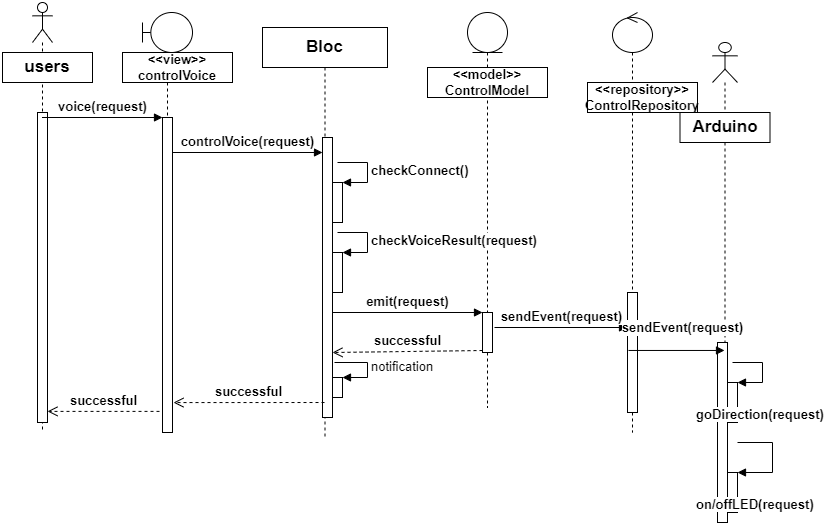
\includegraphics[scale = 0.5]{Hinhve/sequence_dieu_khien_voice.png}
    \caption{Biểu đồ trình tự điều khiển xe bằng giọng nói}
    \label{fig:4.2.2.3}
\end{figure}

Hình \ref{fig:4.2.2.3} thể hiện luồng điều khiển xe bằng giọng nói. Sau khi kết nối được với server, người dùng nói lệnh cho ứng dụng. Tại tầng Bloc sẽ xử lý kết quả giọng nói trước xem câu lệnh có phù hợp hay không, tiếp theo nó sẽ kiểm tra kết nối với server, tiếp đó sẽ gửi tín hiệu với VoiceModel, qua VoiceRepository để gửi sự kiện tới xe Arduino. Arduino lắng nghe sự kiện, nếu sự kiện đúng theo mã đã lập trình, xe thực hiện tắt/bật đèn theo hàm turnOnLed(), turnOffLed() hoặc di chuyển theo hàm goDirection().

 \begin{figure}[H]
    \centering
    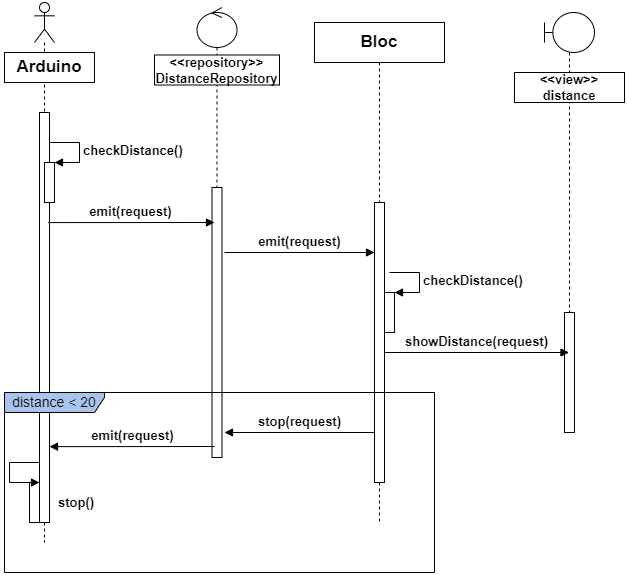
\includegraphics[scale = 0.6]{Hinhve/sequence_gap_vat-can.png}
    \caption{Biểu đồ trình tự xe gặp vật cản}
    \label{fig:4.2.2.4}
\end{figure}

Hình \ref{fig:4.2.2.4} mô tả luồng xe Arduino khi gặp vật cản. Xe Arduino sẽ kiểm tra khoảng cách tới vật trước mặt liên tục và gửi khoảng cách về server. Tại đây, DistanceRepository sẽ nhận được giá trị khoảng cách truyền về, tầng Bloc sẽ kiểm tra khoảng cách, tầng View sẽ hiển thị khoảng cách liên tục, nếu khoảng cách dưới 20 cm sẽ truyền tín hiệu dừng lại, xe Arduino nhận tín hiệu và thực hiện hàm stop().

\subsection{Thiết kế cơ sở dữ liệu}

Trong ĐATN này, em không sử dụng cơ sở dữ liệu.

\subsection{Thiết kế xe Arduino}

Cách ghép nối các module thiết bị lại với nhau.

Nguồn gồm 1 pin được kết nối với Module L298 qua 1 công tắc để tắt/bật nguồn chiếc xe.

Các chân N22, N23, N27, N26 của Module NodeMCU Esp32 được kết nối với mạch cầu L298 giúp điều khiển động cơ xe:
\begin{itemize}
    \item N22 điều khiển bánh xe bên trái đi lùi.
    \item N23 điều khiển bánh xe bên trái đi tiến.
    \item N27 điều khiển bánh xe bên phải đi tiến.
    \item N26 điều khiển bánh xe bên phải đi lùi.
\end{itemize}

Các chân GND là chân của nguồn cấp động cơ xe Arduino. Các chân N22, N23, N27, N6 sẽ tương ứng với IN3, IN4, IN1, IN2 của L298.

\begin{figure}[H]
    \centering
    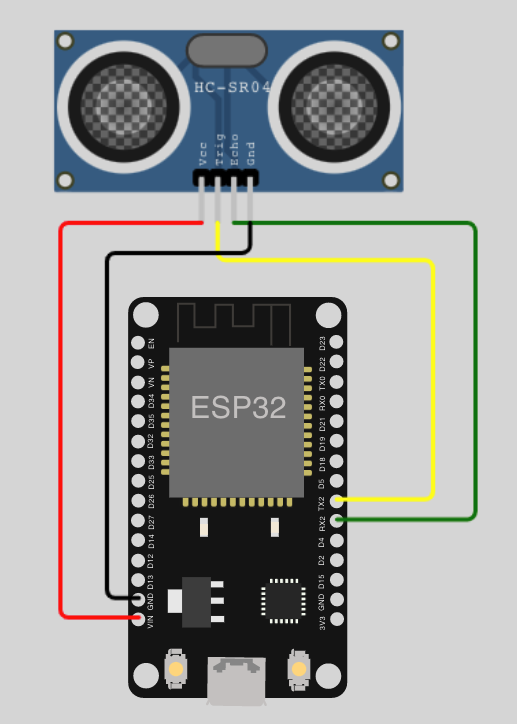
\includegraphics[scale = 0.75]{Hinhve/srhc04-esp32.png}
    \caption{Thiết kế ghép nối module Esp32 với HC-SR04}
    \label{fig:Fig8}
\end{figure}

Ở hình \ref{fig:Fig8}, Module Esp32 được ghép nối với cảm biến siêu âm HC-SR04, chân Echo của cảm biến sẽ được nối với chân N17, chân Trigger sẽ được nối với chân N16, 2 chân VCC, GND sẽ được nối tương ứng với chân Vin, GND của Module Esp32.

\begin{figure}[H]
    \centering
    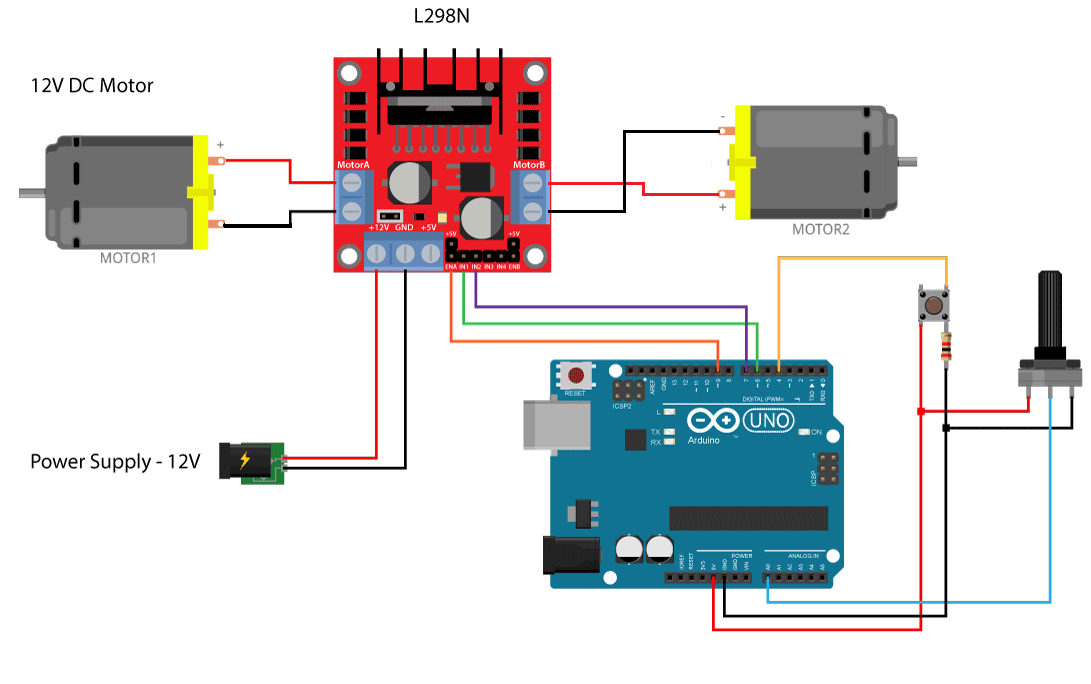
\includegraphics[scale = 0.55]{Hinhve/graft_modules.png}
    \caption{Thiết kế ghép nối các module thiết bị lại với nhau}
    \label{fig:Fig9}
\end{figure}

Hình \ref{fig:Fig9} là mô hình thiết kế ghép nối các Module các thiết bị lại với nhau bao gồm 2 Motor 12V, 1 module L298N, module Esp32, được cấp nguồn từ pin 12V, có công tắc tắt/bật.



\section{Xây dựng ứng dụng}
\subsection{Thư viện và công cụ sử dụng}

Trong quá trình phát triển hệ thống, em đã sử dụng các thư viện mã nguồn mở sau đây:

\begin{table}[H]
\begin{tabular}{| p{4cm} | p{2cm} | p{9cm} |}
\hline
\rowcolor[HTML]{FFCE93} 
\textbf{Mục đích}                & \textbf{Công cụ} & \textbf{Địa chỉ URL}                          \\ \hline
IDE lập trình                    & VSCode           & https://code.visualstudio.com/                \\ \hline
IDE lập trình        & Android Studio        & https://developer.android.com                     \\ \hline
Xây dựng giao diện ứng dụng        & Flutter   & https://flutter.dev \\ \hline
Hỗ trợ realtime & Socket.IO      & https://socket.io   \\ \hline
Hỗ trợ chuyển đổi giọng nói thành chữ                  & speech-to-text        & https://github.com/csdcorp/speech-to-text   \\ \hline
Kết nối ứng dụng với socket                & socket-io-client          & https://github.com/rikulo/socket.io-client-dart                     \\ \hline
\end{tabular}
\caption{Danh sách thư viện hỗ trợ cho ứng dụng và server}
\end{table}

\begin{table}[H]
\begin{tabular}{| p{4cm} | p{2cm} | p{9cm} |}
\hline
\rowcolor[HTML]{FFCE93} 
\textbf{Mục đích}                & \textbf{Công cụ} & \textbf{Địa chỉ URL}                          \\ \hline
IDE lập trình        & Arduino           & https://www.arduino.cc                           \\ \hline
Điều chỉnh đèn LED        & FastLED   & https://github.com/FastLED/FastLED \\ \hline
Hỗ trợ sử dụng thiết bị HC-SR04 đo khoảng cách & HCSR04      & https://github.com/Martinsos/arduino-lib-hc-sr04   \\ \hline
Hỗ trợ đọ mã Json                  & ArduinoJson        & https://github.com/bblanchon/ArduinoJson   \\ \hline
Kết nối Arduino với Socket                & arduino WebSockets          & https://github.com/Links2004/arduinoWebSockets   \\ \hline
Kết nối Arduino với Wifi              & WiFi          & https://github.com/arduino-libraries/WiFi                     \\ \hline
\end{tabular}
\caption{Danh sách thư viện hỗ trợ cho xe Arduino}
\end{table}

\subsection{Kết quả đạt được}

Kết thúc quá trình nghiên cứu ĐATN, em đã đạt được những kết quả sau đây.

\subsubsection{Biết được cách viết một trang web server}

Lĩnh vực IoT ngày càng được ứng dụng rộng rãi, nên việc lập trình viết web là hết sức cần thiết, đặc biệt sử dụng những framework mới. Sau thời gian nghiên cứu, em đã biết cách viết một web server để điều khiển, giám sát trạng thái hoạt động của các thiết bị. Ngoài ra em cũng đã biết cách đẩy một web server lên Heroku - nền tảng đám mây cho phép các lập trình viên xây dựng, triển khai, quản lý và mở rộng ứng dụng. Việc đó giúp cho các thiết bị được kết nối với một server trên Internet mà không phải là server ở dưới localhost.

\subsubsection{Biết được cách viết một ứng dụng đa nền tảng}

Sau khi tìm hiểu và nghiên cứu những framework, ngôn ngữ để xây dựng ứng dụng, em đã lựa chọn Flutter là framework xây dựng ứng dụng của mình. Em đã biết lập trình ngôn ngữ Dart và từ Flutter để chạy được ứng dụng trên 3 nền tảng là Android, iOS và Web. Việc lựa chọn Flutter đem đến những trải nghiệm mượt mà cho người dùng, có thể tiếp cận nhiều nền tảng, thiết bị và giảm chi phí, thời gian cho lập trình viên.

\subsubsection{Biết được cách lắp ráp xe Arduino}

Mặc dù Arduino không nằm trong chuyên ngành Khoa học máy tính mà em theo học, những em đã cố gắng tìm hiểu về các thiết bị, nguyên lý và cách lắp ráp chiếc xe Arduino. Từ đó em đã biết được cách hoạt động của các thiết bị, nối dây giữa các chân mạch, lắp các thành phần lại với nhau để có một chiếc xe hoàn chỉnh, có thể di chuyển các hướng. Ngoài ra xe Arduino còn lắp thêm cảm biến khoảng cách và đèn LED để báo hiệu xe đang gặp vật cản. Xe Arduino là thành phần quan trọng nhất để thực hiện các thao tác mà người dùng sử dụng ứng dụng.

\subsubsection{Biết được cách truyền - nhận thông tin bằng Socket.IO}

Ngày nay, trải nghiệm người dùng đang là vấn đề nhiều hệ thống hướng tới. Một trong những trải nghiệm tốt với người dùng là thời gian phản hồi nhanh, thời gian thực. Vì vậy em đã lựa chọn Socket.IO và biết cách thêm vào ứng dụng, server và mã nguồn của thiết bị để nhận tín hiệu của nhau. Việc này đã xử lý được vấn đề thời gian thực giữa ứng dụng và thiết bị. 

\subsubsection{Biết được cách kết nối và lập trình giữa Module ESP32 với ứng dụng đa nền tảng}

Sau khi đã lắp đặt xong xe Arduino, lập trình xong web server và biết cách tạo ứng dụng bằng Flutter, em đã biết cách kết nối giữa xe Arduino với Flutter thông qua server, từ đó em lập trình đưa các tín hiệu từ ứng dụng để xe Arduino có thể hiểu và di chuyển, thực hiện một số chức năng đặc biệt khác. Việc kết nối và lập trình này chính là phần chính để các thiết bị có thể lắng nghe được nhau và hoạt động một cách mượt mà. Từ đó, đồ án IoT của em đã được hoàn thiện đầy đủ.


Các thông tin về ứng dụng của em:
\begin{itemize}
    \item Dung lượng toàn bộ mã nguồn: 1.3 GB.
    \item Dung lượng ứng dụng đa nền tảng: 32MB.
\end{itemize}

\subsection{Minh họa các chức năng chính}

Dưới đây là ảnh minh hoạ một số chức năng chính của hệ thống.

\subsubsection{Điều khiển xe di chuyển}

\begin{figure}[H]
    \centering
    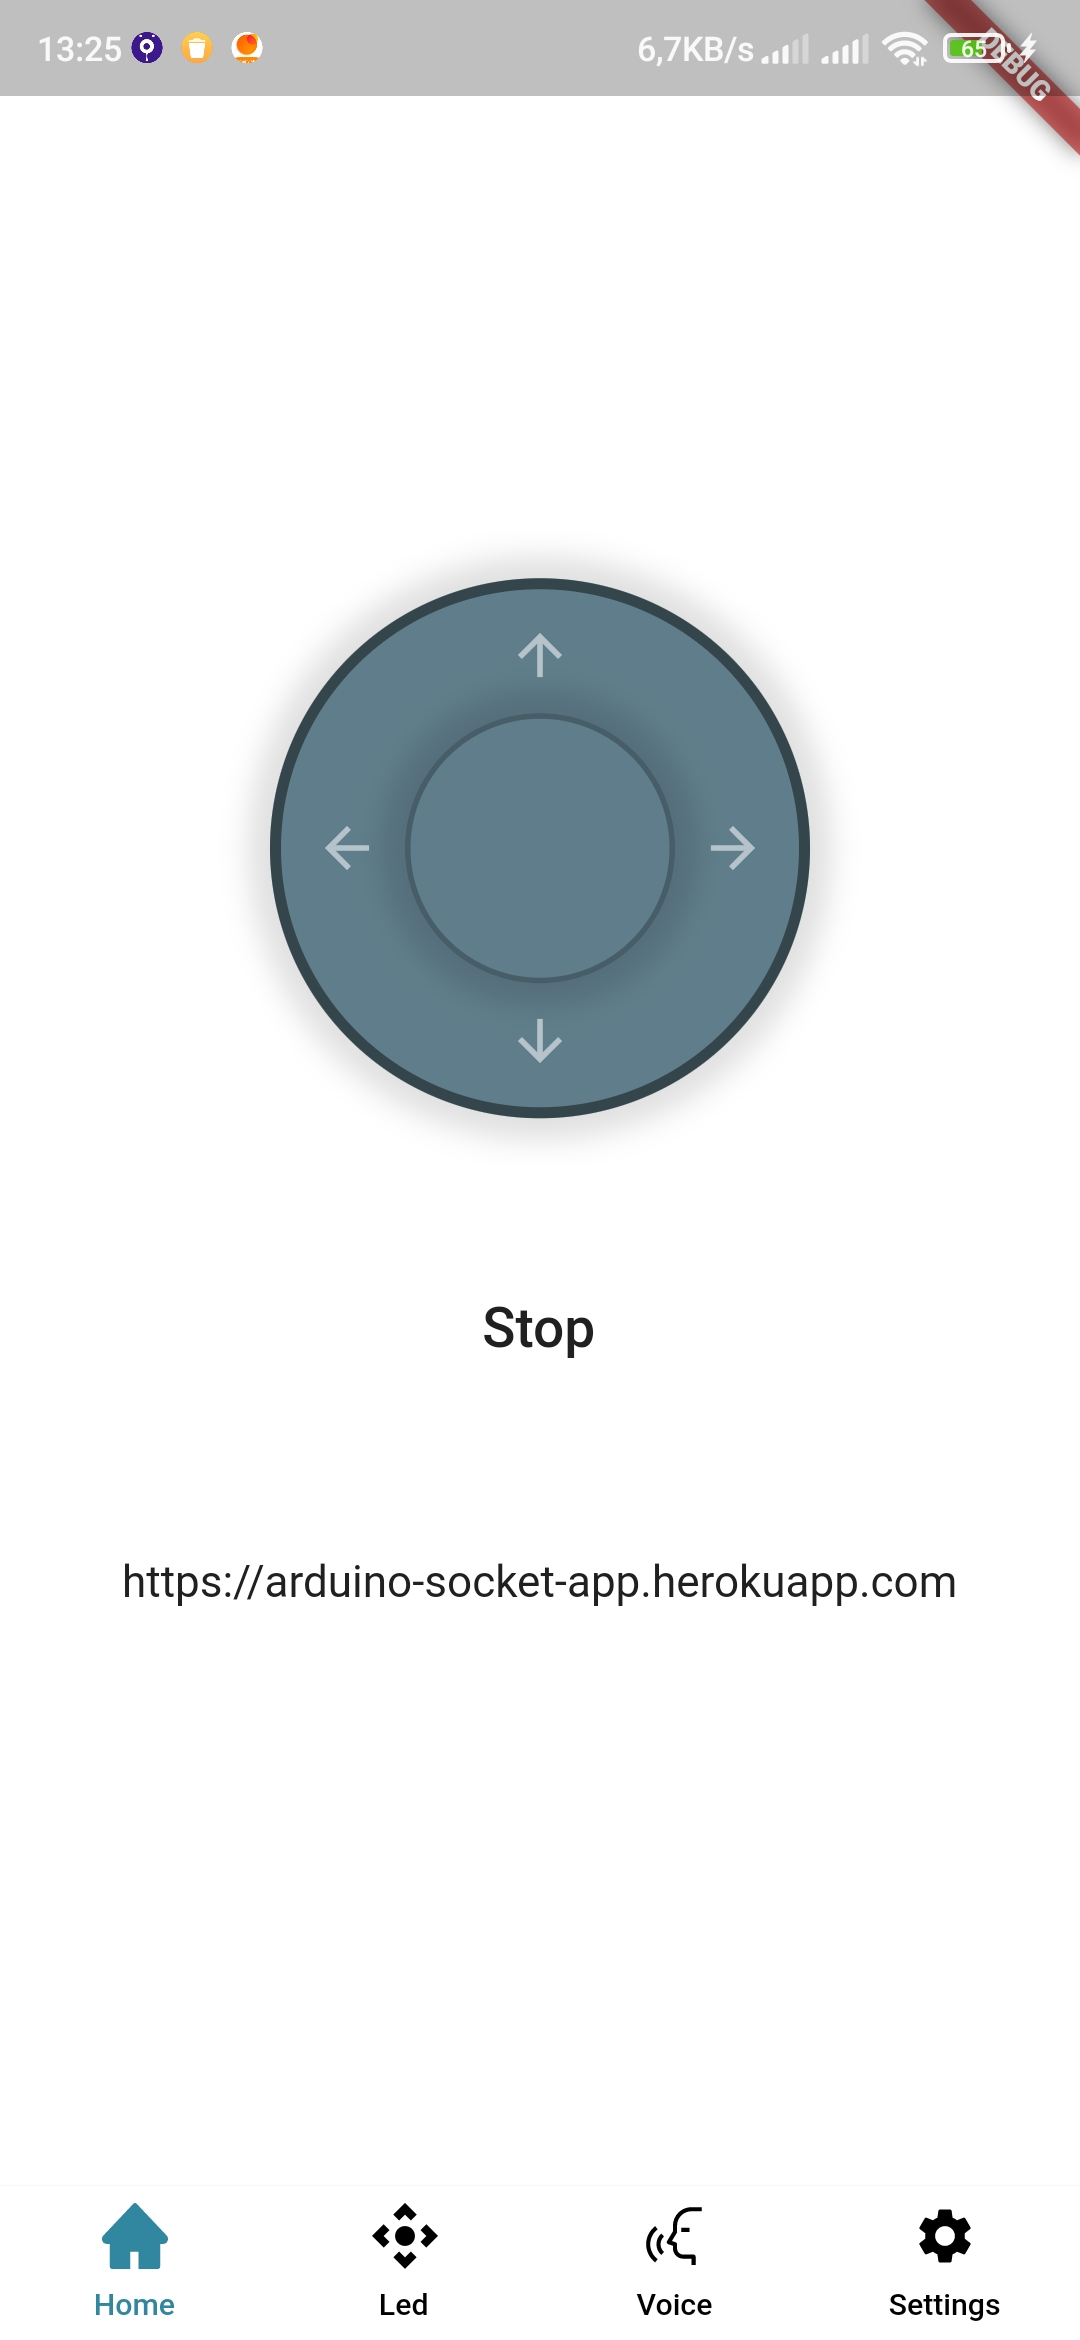
\includegraphics[scale = 0.2]{Hinhve/app_1.jpg}
    \caption{Hình ảnh màn trang chủ - màn điều khiển xe}
    \label{fig:Fig9}
\end{figure}

Hình \ref{fig:Fig9} là hình ảnh màn điều khiển xe của ứng dụng Flutter, người dùng sẽ sử dụng bộ điều khiển ở giữa màn hình để điều khiển các hướng.

\subsubsection{Điều khiển đèn LED}

\begin{figure}[H]
    \centering
    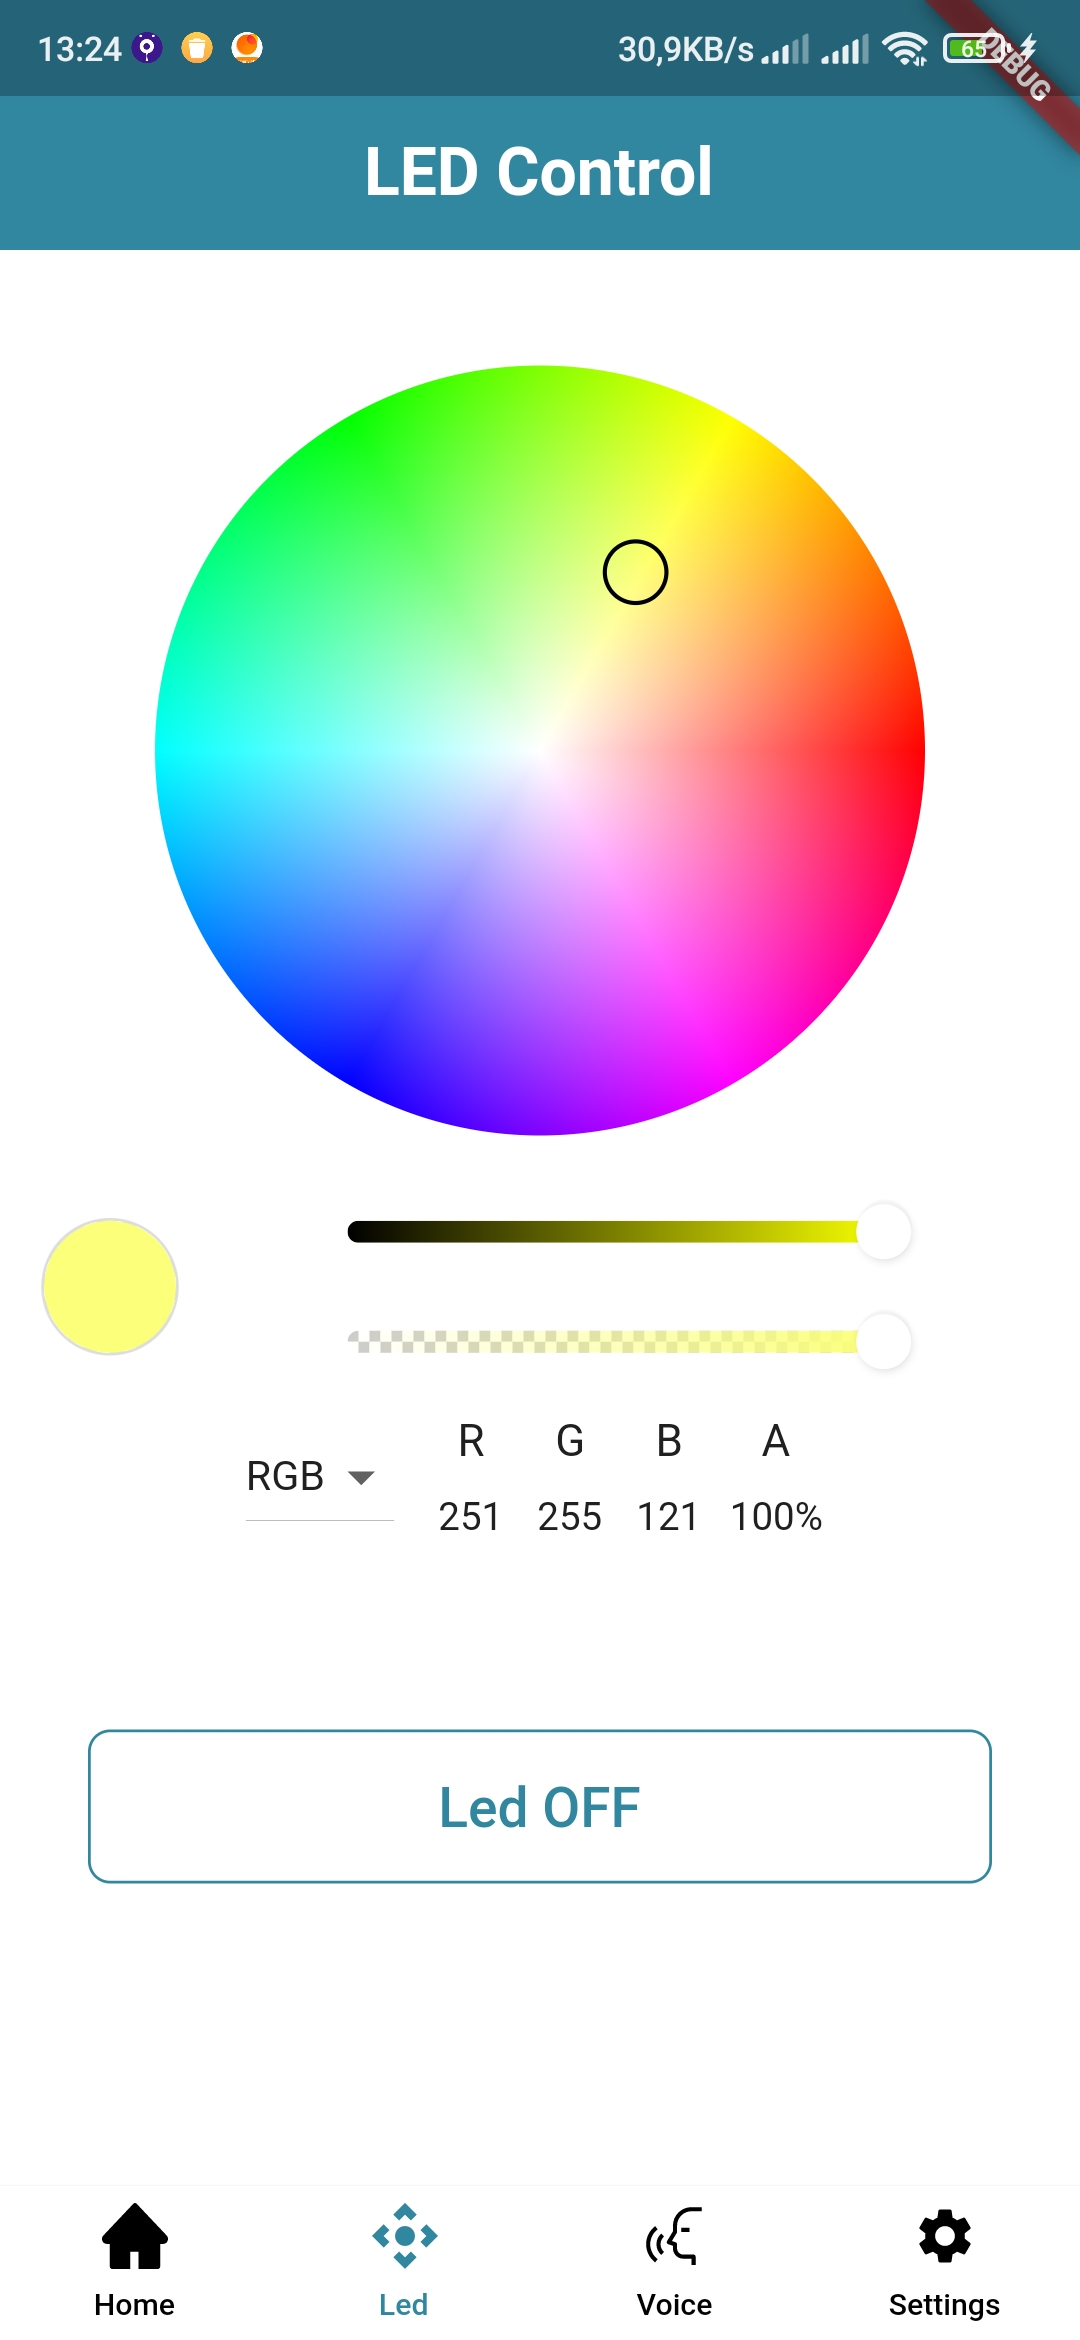
\includegraphics[scale = 0.2]{Hinhve/app_2.jpg}
    \caption{Hình ảnh màn điều khiển đèn LED}
    \label{fig:Fig10}
\end{figure}

Hình \ref{fig:Fig10} là hình ảnh màn điều khiển đèn LED, người dùng có thể chỉnh sửa màu của đèn LED đủ tất cả mã màu, sau đó ấn nút Led OFF để bật đèn lên theo màu đã chọn.

\subsubsection{Điều khiển xe bằng giọng nói}

\begin{figure}[H]
    \centering
    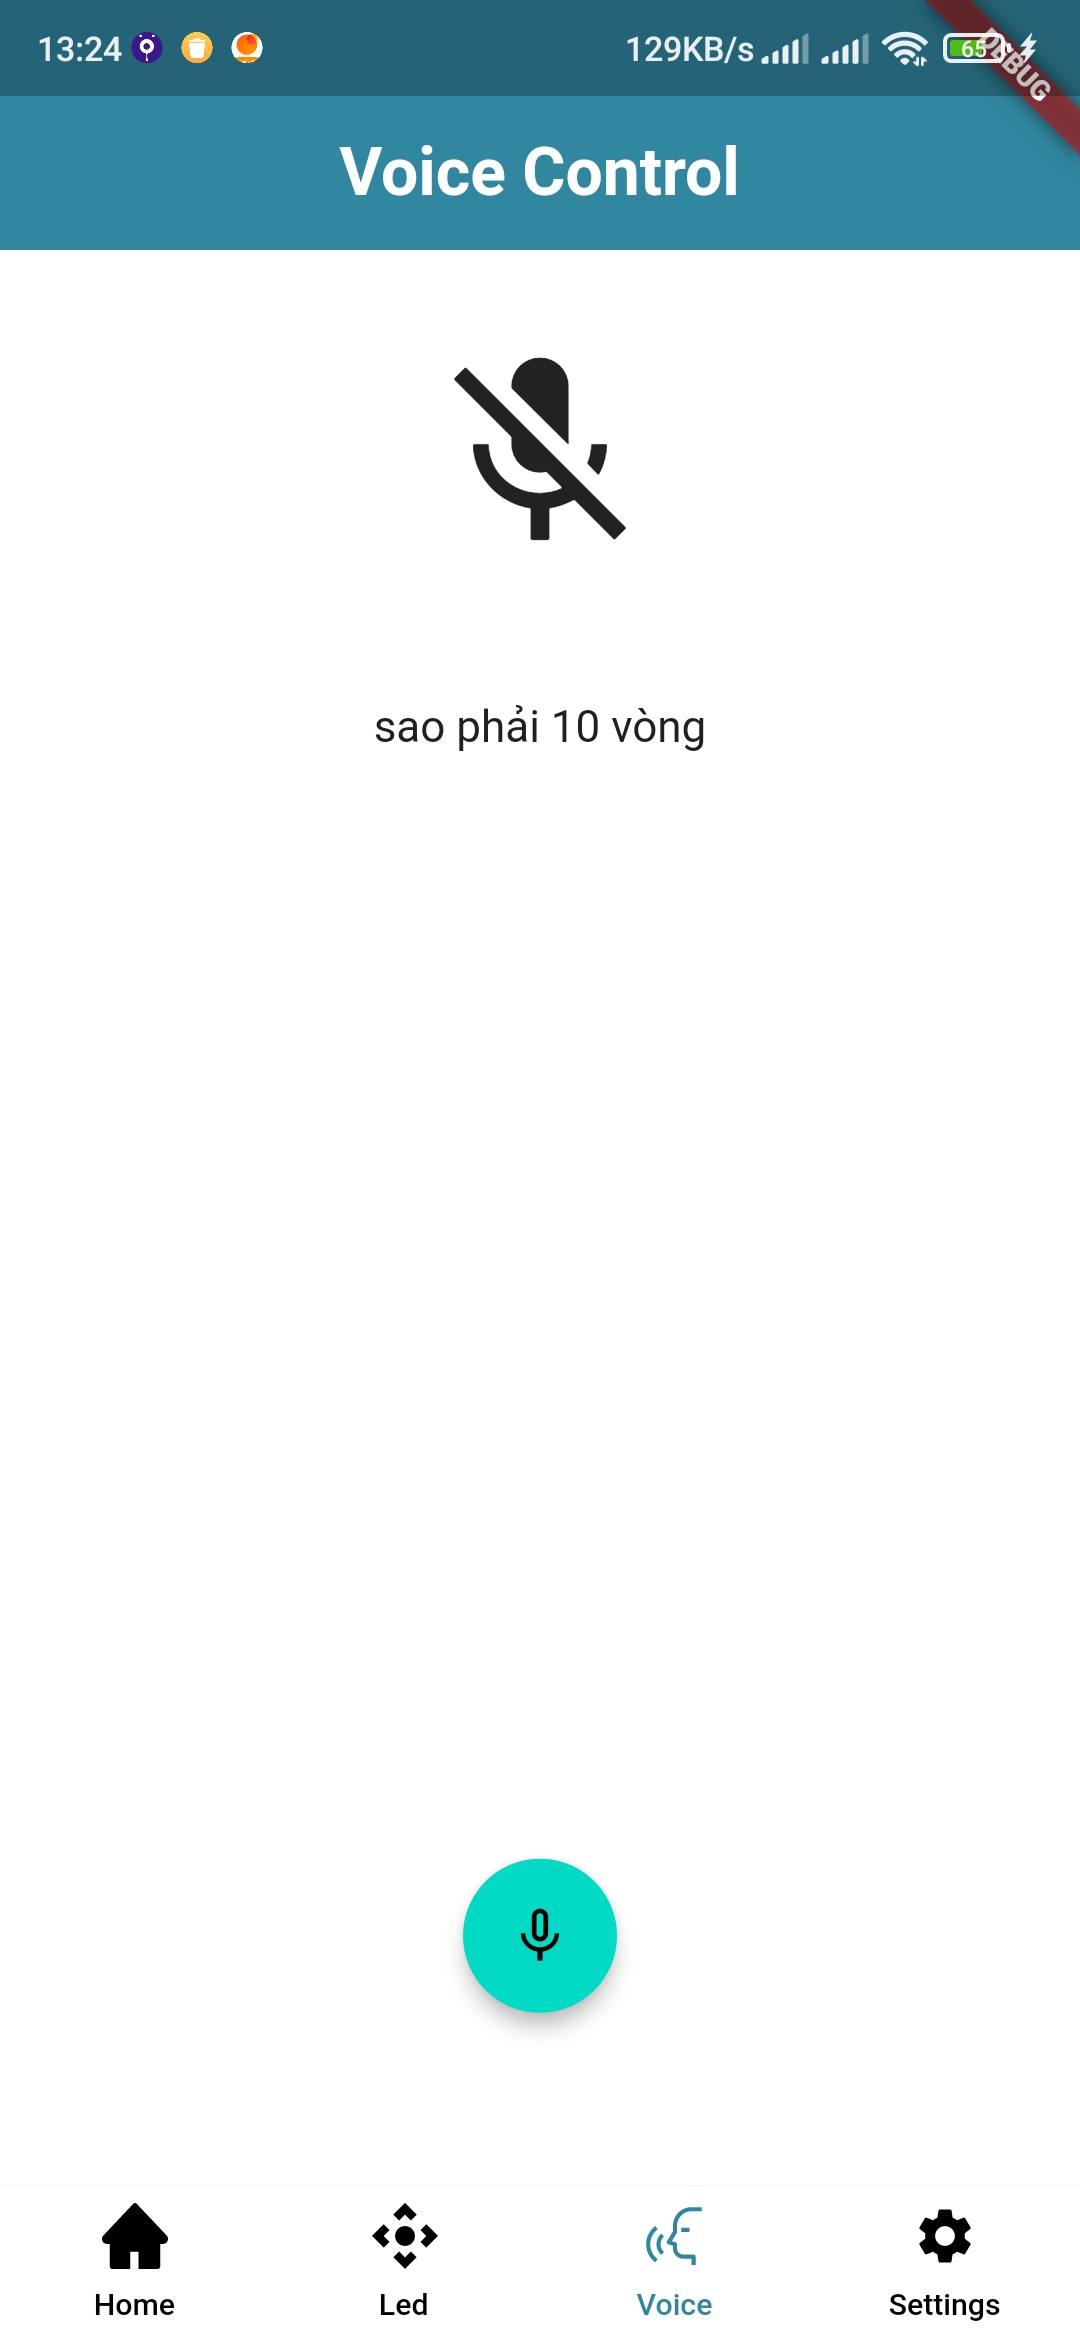
\includegraphics[scale = 0.2]{Hinhve/app_3.jpg}
    \caption{Hình ảnh màn điều khiển bằng giọng nói}
    \label{fig:Fig11}
\end{figure}

Hình \ref{fig:Fig11} là hình ảnh màn điều khiển xe Arduino bằng giọng nói, người dùng sẽ nói một số câu lệnh đơn giản để ứng dụng phân tích, gửi đến xe và xe thực hiện yêu cầu đó.

\subsubsection{Các tính năng thêm và hướng dẫn}

\begin{figure}[H]
    \centering
    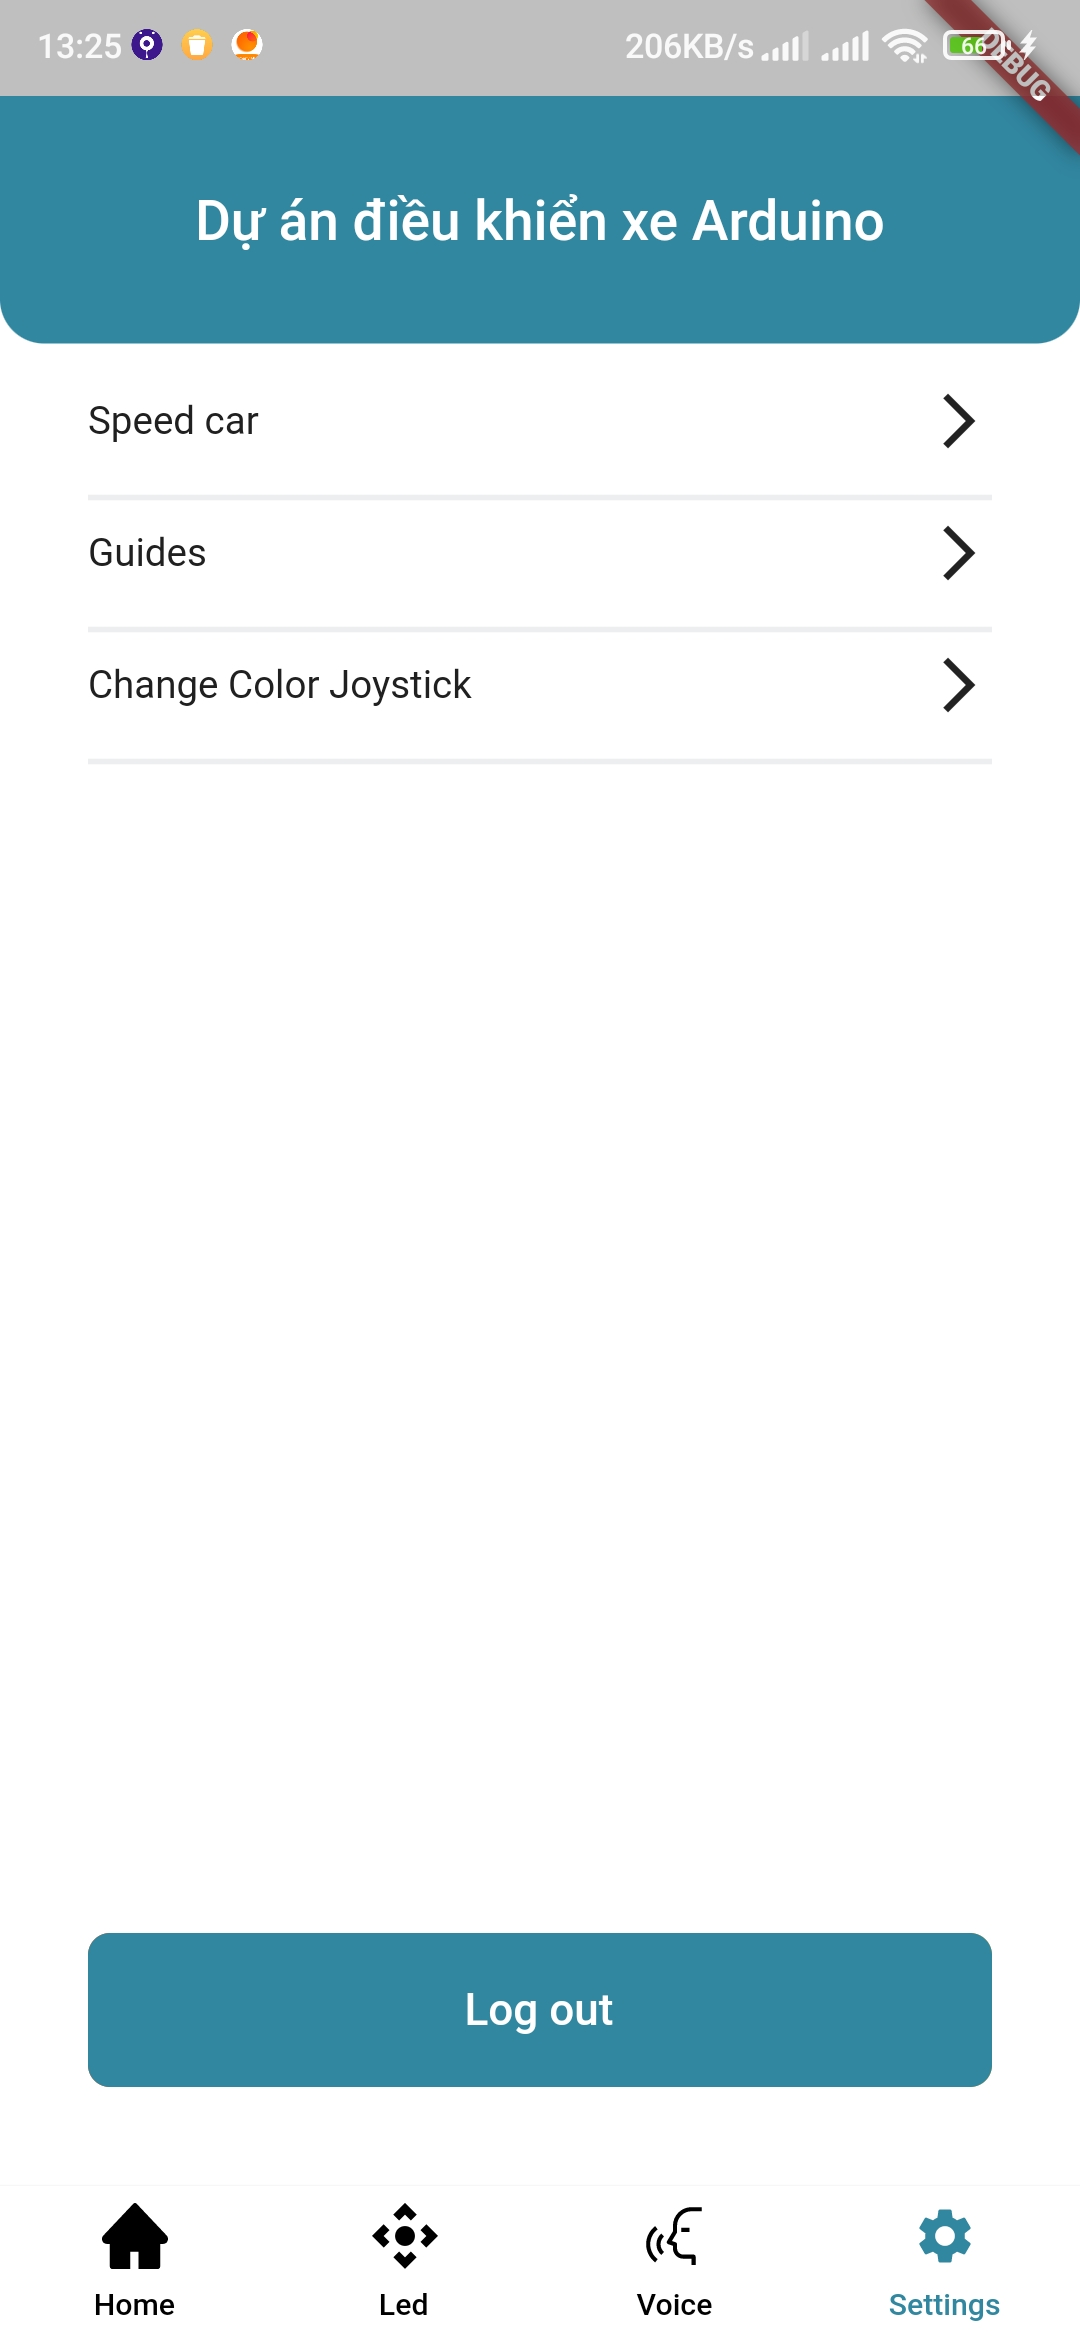
\includegraphics[scale = 0.2]{Hinhve/app_4.jpg}
    \caption{Hình ảnh màn một số tính năng thêm}
    \label{fig:Fig12}
\end{figure}

Hình \ref{fig:Fig12} là hình ảnh một số chức năng thêm, người dùng có thể tuỳ chỉnh sửa như: tốc độ của xe, hướng dẫn kết nối, thay đổi màu sắc bộ điều khiển.

\subsubsection{Xe Arduino}

Các hình \ref{fig:Fig13} \ref{fig:Fig14} \ref{fig:Fig15} là hình ảnh mô hình Arduino các mặt có gắn cảm biến khoảng cách, xe bao gồm 2 bánh động cơ và 1 bánh điều hướng.

\begin{figure}[H]
    \centering
    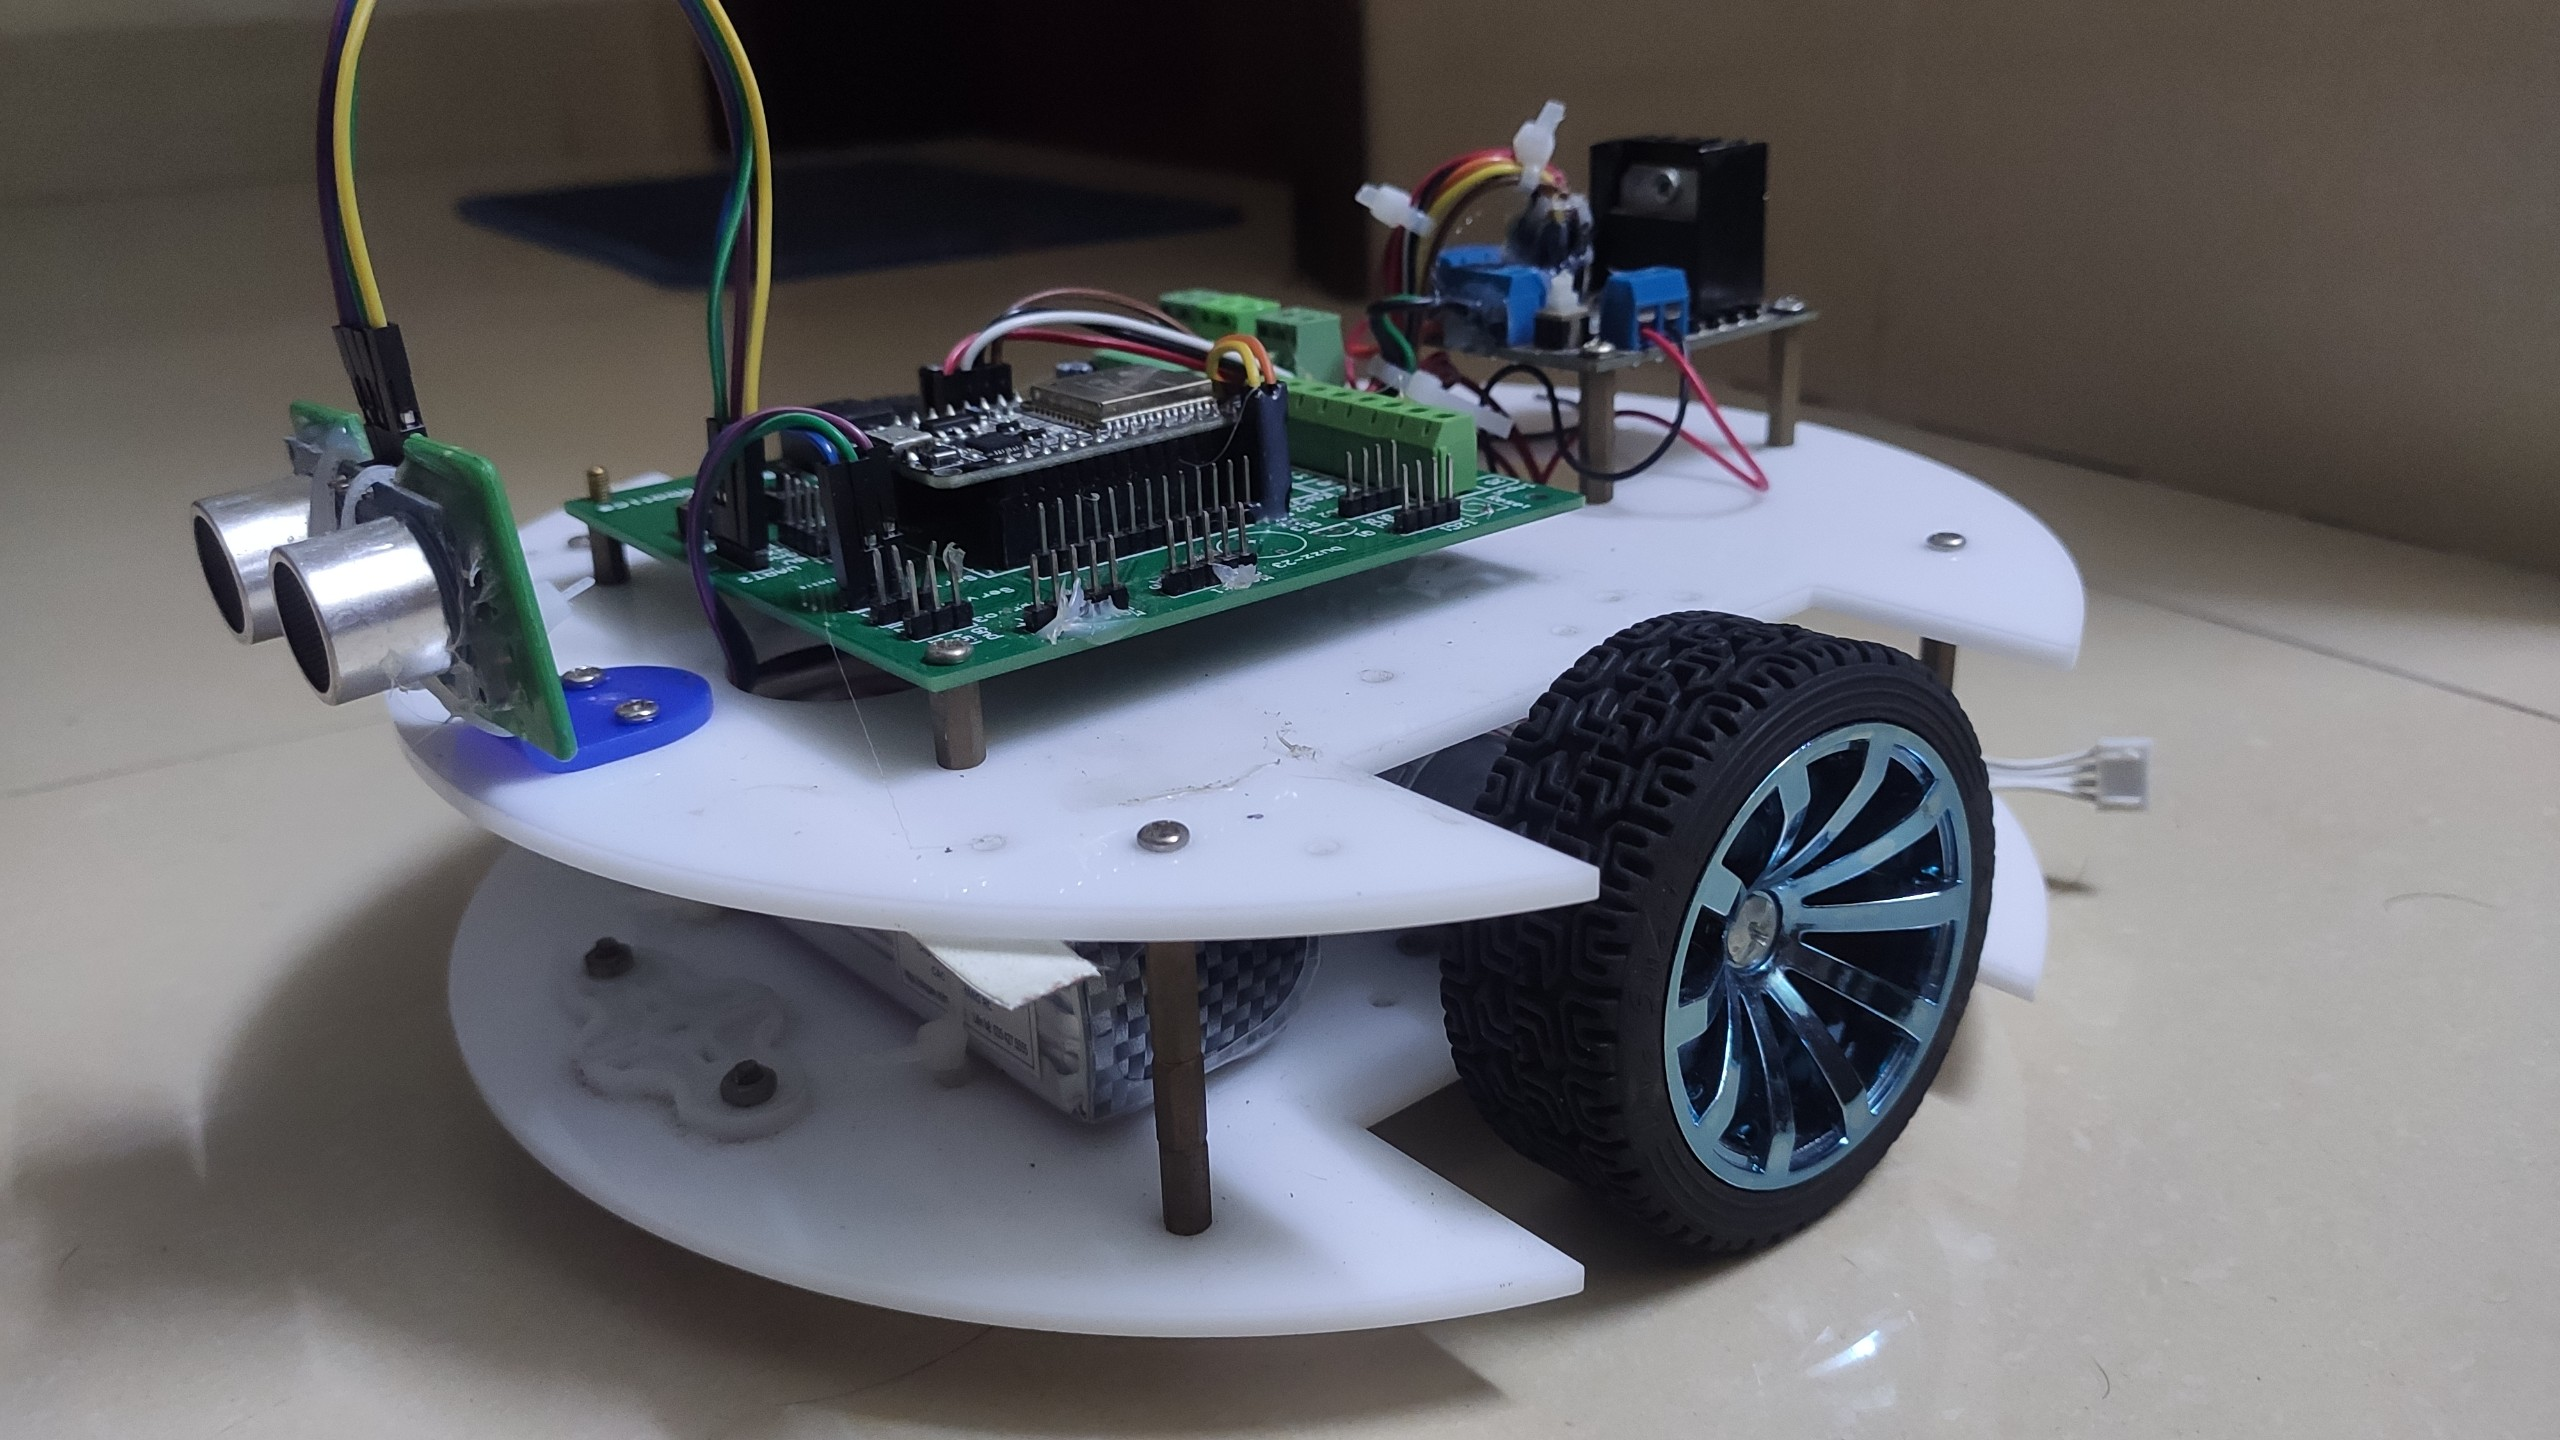
\includegraphics[scale = 0.15]{Hinhve/car_1.jpg}
    \caption{Hình ảnh xe Arduino mặt bên}
    \label{fig:Fig13}
\end{figure}

\begin{figure}[H]
    \centering
    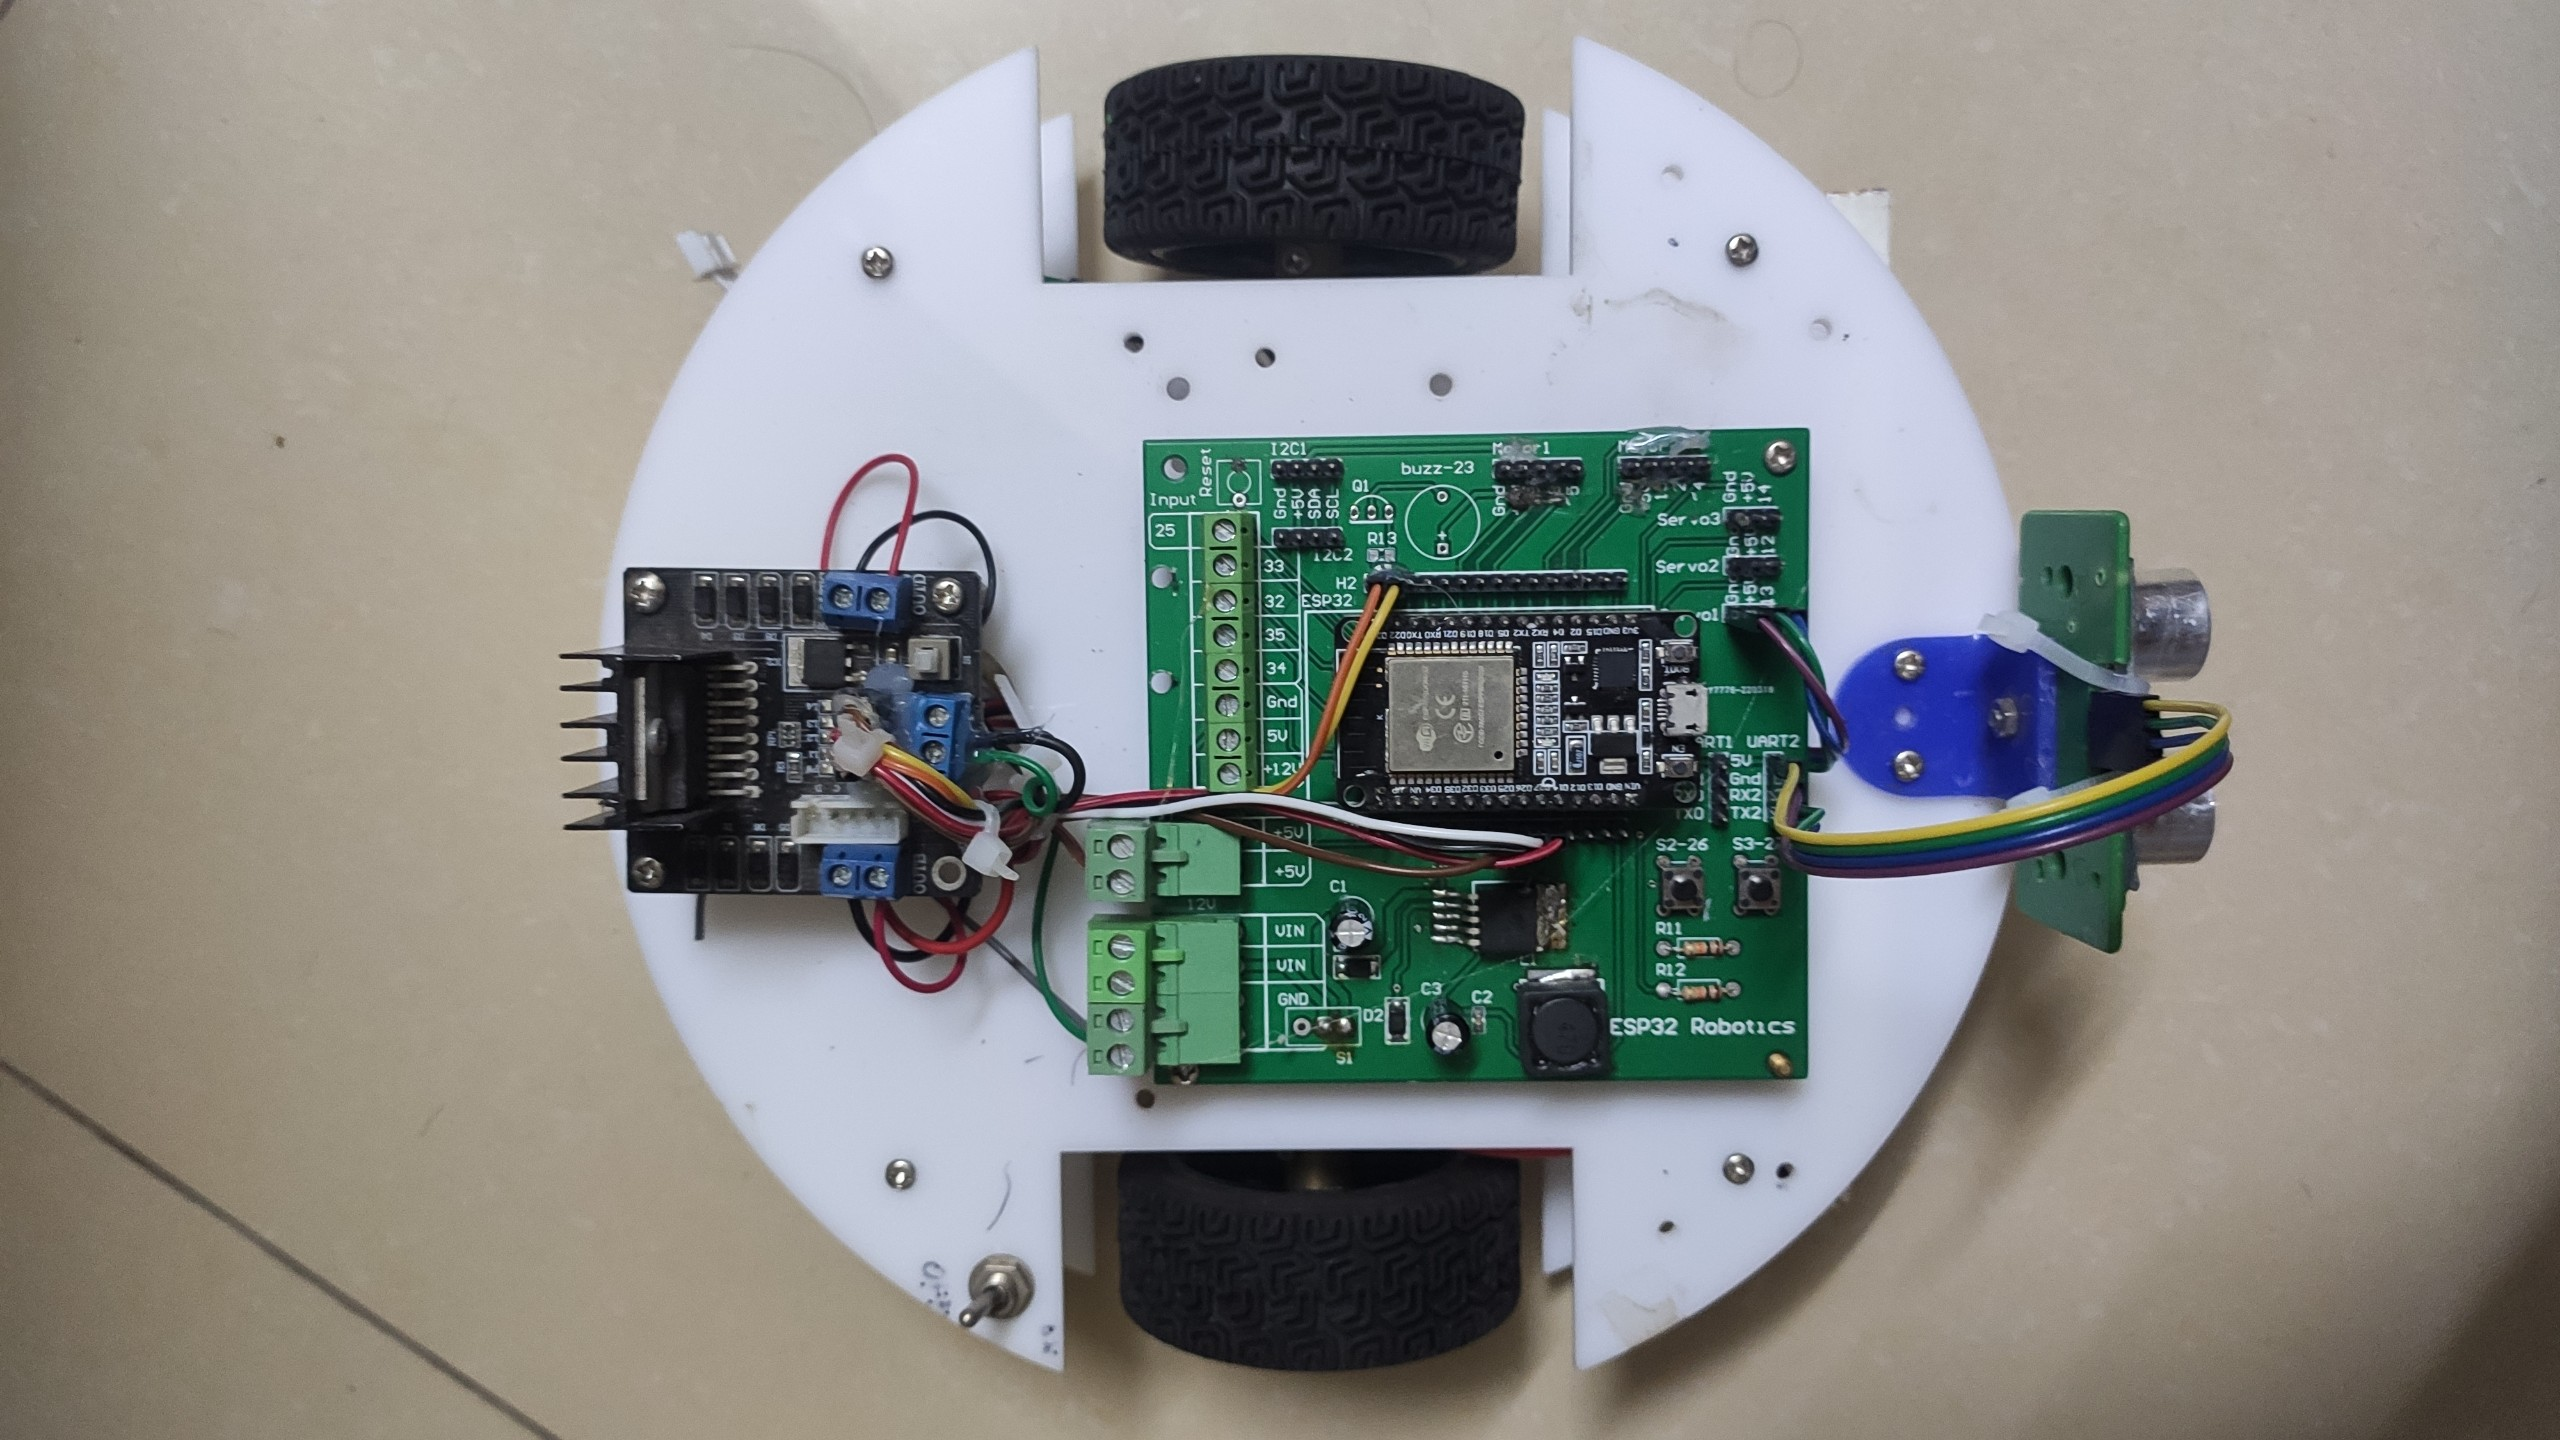
\includegraphics[scale = 0.15]{Hinhve/car_2.jpg}
    \caption{Hình ảnh xe Arduino mặt trên}
    \label{fig:Fig14}
\end{figure}

\begin{figure}[H]
    \centering
    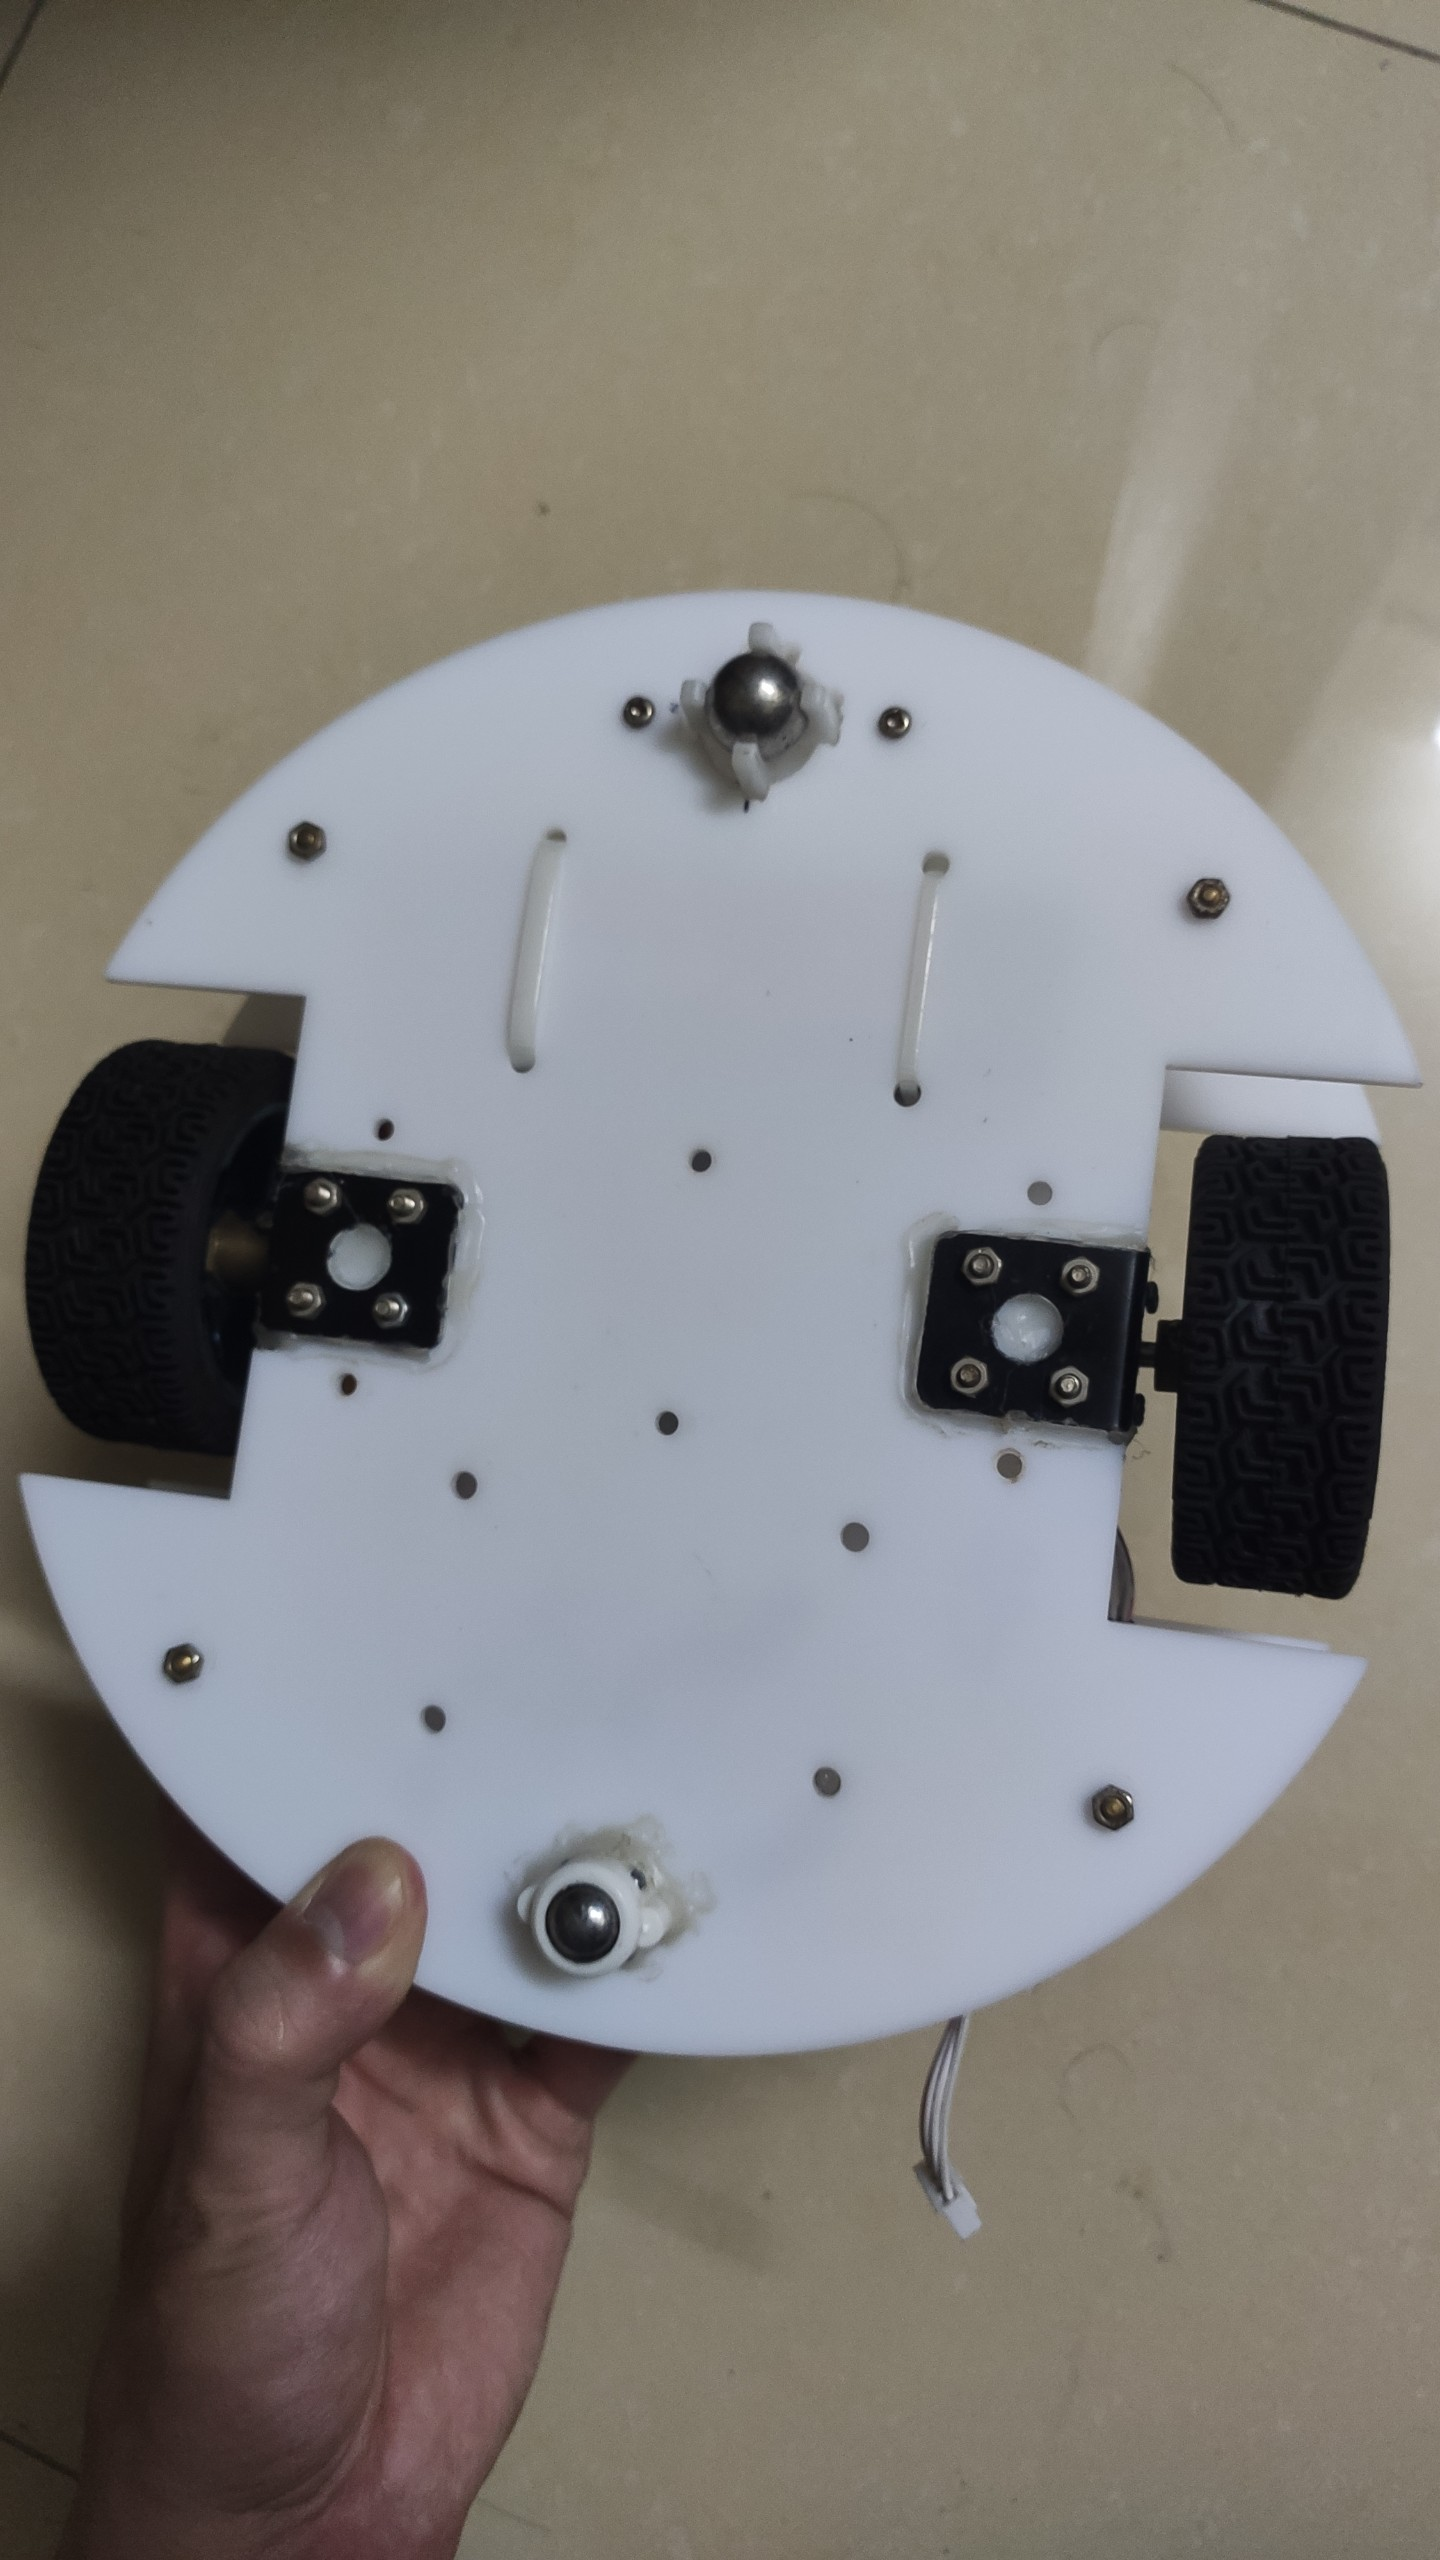
\includegraphics[scale = 0.15]{Hinhve/car_3.jpg}
    \caption{Hình ảnh xe Arduino mặt dưới}
    \label{fig:Fig15}
\end{figure}

\section{Kiểm thử}

Trong quá trình thực hiện ĐATN, em đã thực hiện kiểm thử hệ thống và đã kiểm thử các chức năng chính: Đăng nhập, kết nối với server, điều khiển xe đi các hướng, điều khiển đèn, điều khiển bằng giọng nói, thay đổi tốc độ xe, gặp vật cản, đăng xuất. Em đã thực hiện kiểm thử trên cả 3 nền tảng là Android, iOS, Web và đều đạt.

Một số kiểm thử em đã thực hiện sẽ được trình bày dưới đây.

\subsection{Kiểm thử chức năng đăng nhập, đăng xuất}

\begin{table}[H]
\begin{tabular}{| p{3cm} | p{4cm} | p{5cm} | p{2cm} |}
\hline
\rowcolor[HTML]{FFCE93} 
\textbf{Chức năng} & \textbf{Giá trị đầu vào}       & \textbf{Giá trị đầu ra mong muốn}                            & Kết quả \\ \hline
Đăng nhập          & Chỉ nhập địa chỉ server hoặc nhập port  & Thông báo cần nhập đủ thông tin                               & đạt     \\ \hline
Đăng nhập          & Nhập đúng địa chỉ server và port & thông báo đăng nhập thành công, hiển thị trang chủ           & đạt     \\ \hline
Đăng xuất          & Nhấn vào đăng xuất             & thực hiện đăng xuất khỏi hệ thống, trở về màn hình đăng nhập & đạt     \\ \hline
\end{tabular}
\caption{Bảng kiểm thử chức năng đăng nhập, đăng xuất}
\end{table}

\subsection{Kiểm thử chức năng điều khiển xe các hướng}

\begin{table}[H]
\begin{tabular}{| p{3cm} | p{4cm} | p{5cm} | p{2cm} |}
\hline
\rowcolor[HTML]{FFCE93} 
\textbf{Chức năng} & \textbf{Giá trị đầu vào}       & \textbf{Giá trị đầu ra mong muốn}                            & Kết quả \\ \hline
Xe đi thẳng          & Di con trỏ lên trên  & Xe di chuyển đi thẳng                               & đạt     \\ \hline
Xe rẽ phải          & Di con trỏ sang phải & Xe di chuyển sang phải           & đạt     \\ \hline
Xe rẽ trái          & Di con trỏ sang trái             & Xe di chuyển sang trái & đạt     \\ \hline
Xe đi lùi          & Di con trỏ xuống dưới             & Xe di chuyển đi lùi & đạt     \\ \hline
Thay đổi tốc độ xe          & Nhập lại tốc độ xe từ 0 đến 255             & Xe di chuyển tốc độ đã cài đặt & đạt     \\ \hline
\end{tabular}
\caption{Bảng kiểm thử chức năng điều khiển xe các hướng}
\end{table}

\subsection{Kiểm thử chức năng điều khiển đèn LED}

\begin{table}[H]
\begin{tabular}{| p{3cm} | p{4cm} | p{5cm} | p{2cm} |}
\hline
\rowcolor[HTML]{FFCE93} 
\textbf{Chức năng} & \textbf{Giá trị đầu vào}       & \textbf{Giá trị đầu ra mong muốn}                            & Kết quả \\ \hline
Bật đèn LED          & Nhấn vào nút để nút sáng lên  & Đèn sáng lên                               & đạt     \\ \hline
Tắt đèn LED          & Nhấn vào nút để nút tối đi & Đèn tắt đi           & đạt     \\ \hline
\end{tabular}
\caption{Bảng kiểm thử chức năng điều khiển đèn LED}
\end{table}

\subsection{Kiểm thử chức năng điều khiển bằng giọng nói}

\begin{table}[H]
\begin{tabular}{| p{3cm} | p{4cm} | p{5cm} | p{2cm} |}
\hline
\rowcolor[HTML]{FFCE93} 
\textbf{Chức năng} & \textbf{Giá trị đầu vào}       & \textbf{Giá trị đầu ra mong muốn}                            & Kết quả \\ \hline
Di chuyển          & Đọc hướng di chuyển & Xe di chuyển theo hướng đã đọc                               & đạt     \\ \hline
Di chuyển nhiều vòng          & Đọc hướng di chuyển và số vòng & Xe di chuyển theo hướng và số vòng đã đọc          & đạt     \\ \hline
Di chuyển          & Đọc sai hướng di chuyển hoặc đọc từ khác             & Thông báo cần đọc lại & đạt     \\ \hline
Tắt/bật đèn LED & Đọc trạng thái tắt/bật             & Đèn tắt/bật & đạt    \\ \hline
\end{tabular}
\caption{Bảng kiểm thử chức năng điều khiển bằng giọng nói}
\end{table}

\subsection{Kiểm thử chức năng cảm biến khoảng cách}

\begin{table}[H]
\begin{tabular}{| p{3cm} | p{4cm} | p{5cm} | p{2cm} |}
\hline
\rowcolor[HTML]{FFCE93} 
\textbf{Chức năng} & \textbf{Giá trị đầu vào}       & \textbf{Giá trị đầu ra mong muốn}                            & Kết quả \\ \hline
Dừng khi gặp vật cản          & Di chuyển và gặp vật cản cách khoảng 20cm & Xe dừng lại và báo đèn đỏ & đạt    \\ \hline
Đo khoảng cách trước mặt          & Khoảng cách giữa xe và vật cản trước mặt & Hiển thị khoảng cách lên màn hình          & đạt     \\ \hline
\end{tabular}
\caption{Bảng kiểm thử chức năng cảm biến khoảng cách}
\end{table}

\section{Triển khai}

Ở phần này, em xin trình bày mô hình và cách thức triển khai hệ thống của mình. Ứng dụng của em chia làm 3 phần:

\begin{itemize}
    \item Phần thứ nhất là xe Arduino, xe được lắp đặt dựa trên Module ESP32 chịu trách nhiệm xử lý thông tin, quản lý các module khác.
    \item Phần thứ hai là web server, hiện tại server để chạy được hệ thống đang chạy trên máy chủ Windows 10, tốc độ phản hồi nhanh, chưa tới 1 giây.
    \item Phần thứ ba là ứng dụng Flutter, ứng dụng chạy được trên thiết bị Android, iOS và nền tảng Web. Ứng dụng có tính linh hoạt về giao diện nên có thể chạy trên nhiều thiết bị mà không bị vỡ hình hay bị sai kích thước.
\end{itemize}

\end{document}
